\documentclass[12pt]{zettel}

\usepackage{multicol}

%\renewcommand{\gregor}{\put(10.0,-3.5){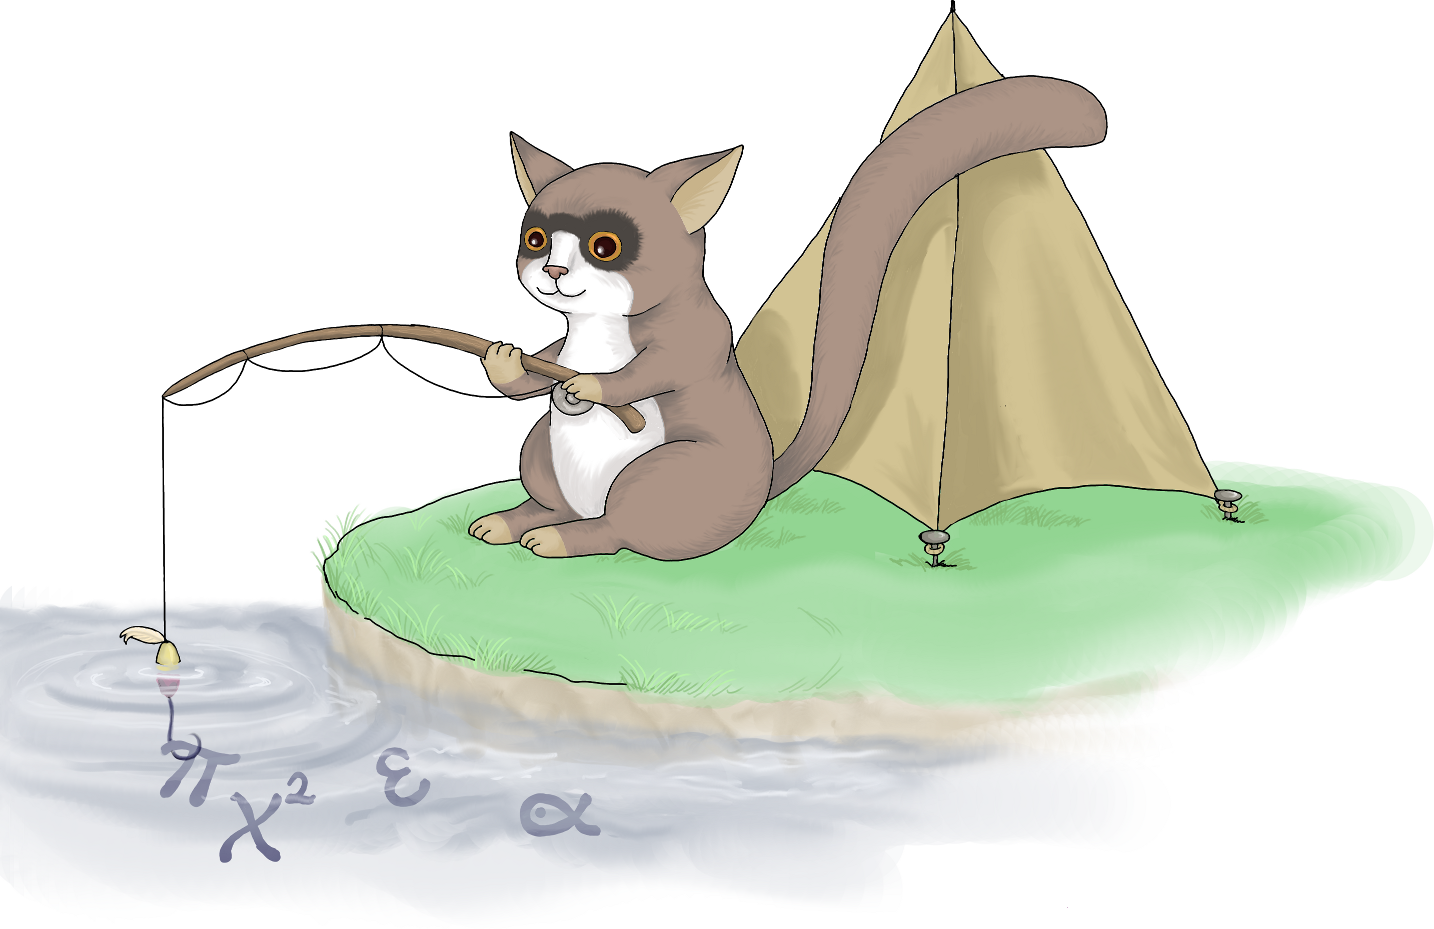
\includegraphics[scale=0.18]{campgregor}}}

\usepackage{framed}
\definecolor{shadecolor}{rgb}{.97,.97,.97}

\geometry{tmargin=1.5cm,bmargin=1.5cm,lmargin=2.9cm,rmargin=2.9cm}

\renewcommand{\gregor}{\put(9.2,-3.5){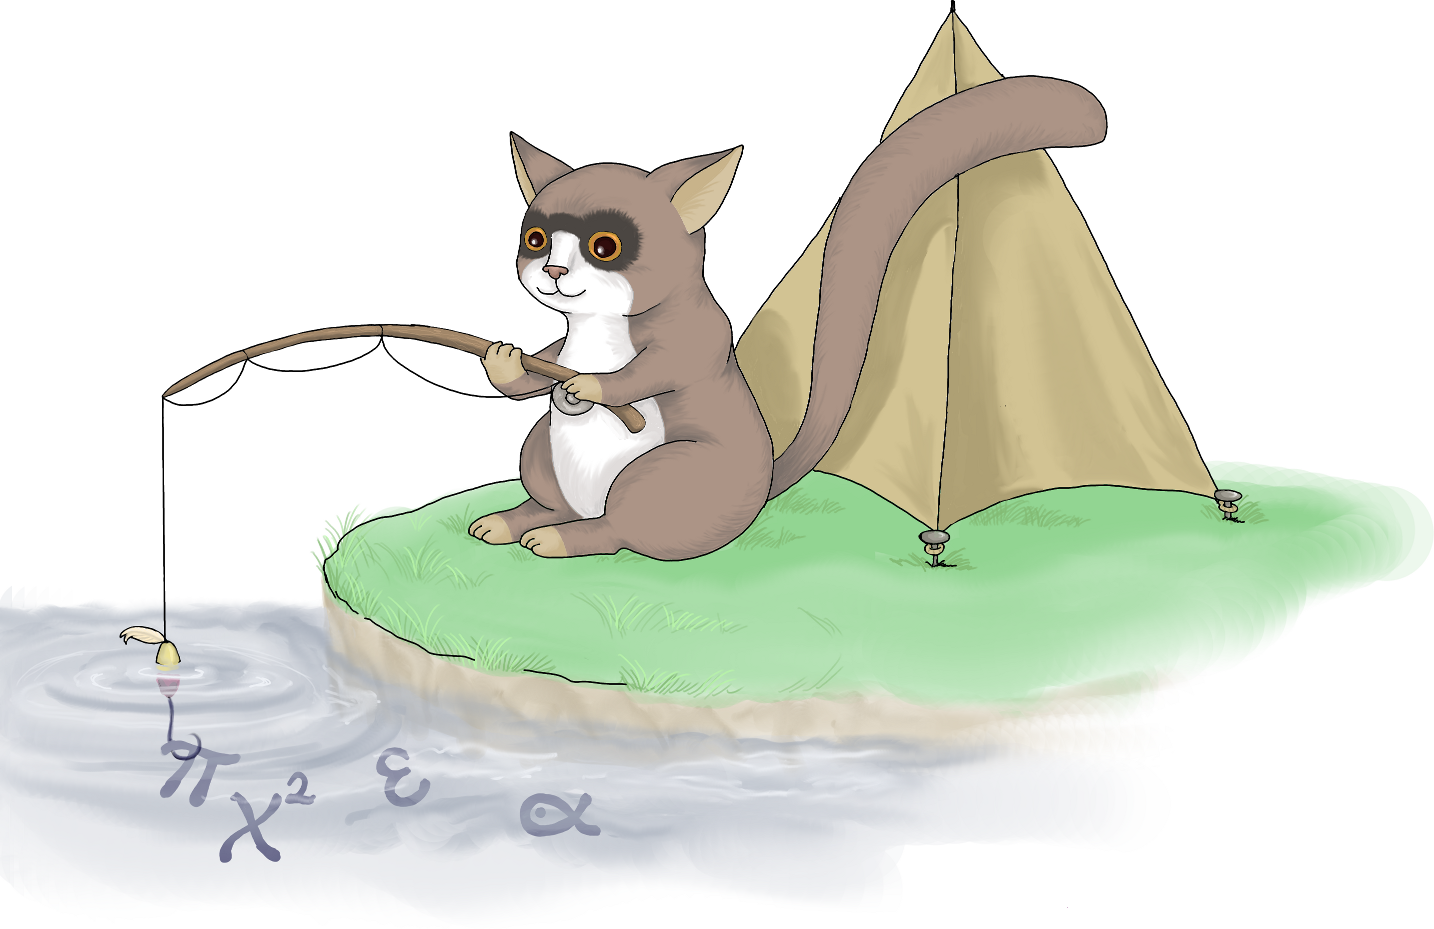
\includegraphics[scale=0.16]{campgregor}}}
\begin{document}

\renewcommand{\betreff}{Mathecamp des Matheschülerzirkels Augsburg}

\makeletterhead{}
\vspace{-2em}

Liebe Schülerinnen und Schüler, liebe Eltern,

wir freuen uns sehr, dass ihr mit uns aufs Mathecamp
fahrt. Unten stehen ein paar Informationen für euch und eure Eltern, bevor es
am 16.~August dann los geht.

Wir bedanken uns herzlich bei \emph{Bündnis für Augsburg}, dem
\emph{Mathematisch-Physikalischen Verein} und den Professorinnen und
Professoren der Lehrstühle für \emph{Algebra und Zahlentheorie},
\emph{Angewandte Analysis} und \emph{Nichtlineare Analysis} des Instituts für
Mathematik für ihre Unterstützung.

Besonderer Dank gebührt einem Professor des
Lehrstuhls für \emph{Analysis und Geometrie}, ohne dessen engagierten Einsatz
das Mathecamp nicht denkbar gewesen wäre.

Ferner bedanken wir uns bei Ihnen, liebe Eltern, für die zahlreichen
Spenden.

Wir sehen uns am 16. August! Wenn ihr in der Zwischenzeit Fragen habt, zögert
nicht, uns anzuschreiben oder anzusprechen.

\vspace{1em}

Euer Team vom Mathezirkel

%{\small Meru Alagalingam, Martin Baur, Ingo Blechschmidt, Tim Dafler, Philipp Düren,
%Alexander Engel, Kathrin Helmsauer, Christian Hübschmann, Jil Hümmer, Sven Prüfer,
%Lisa Reischmann, Peter Uebele}

{\small Meru Alagalingam, Tim Baumann, Martin Baur, Ingo Blechschmidt, Tim
Dafler, Philipp Düren, Alexander Engel, Johanna Fleckenstein, Kathrin
Helmsauer, Prof. Dr. Marco Hien, Christian Hübschmann, Jil Hümmer, Simon
Kapfer, Sven Prüfer, PD Dr. Peter Quast, Lisa Reischmann, Peter Uebele, Prof.
Dr. Timo Schürg, Carina Willbold, Christopher Wulff, Stephanie Zapf}

\begin{shaded}
\textbf{Anreise per Bus.} Falls ihr auf der Anmeldung angegeben habt, dass ihr mit dem
Mathezirkelbus nach Violau fahren möchtet, kommt bitte am 16. August um
9:30 Uhr zum Messeparkplatz bei der Uni Augsburg: Universitätsstr. 16, 86159
Augsburg. Karte: \url{https://goo.gl/maps/h4lBY}

\textbf{Individuelle Anreise.} Falls ihr nicht mit uns nach Violau fahrt, kommt
zwischen 10:00 Uhr und 11:00 Uhr direkt zum Bruder-Klaus-Heim:
St. Michael Straße 15, 86450 Violau-Altenmünster. Anfahrt:
\url{http://tiny.cc/3lxrjx}

Wenn ihr nicht mehr sicher seid, was ihr bei der Anmeldung angegeben habt,
schickt uns einfach eine kurze Mail.
\end{shaded}

\begin{shaded}
\textbf{Kontakt.} Für Fragen und Notfälle stehen wir euch jederzeit zur
Verfügung. \textbf{XXX: Das negativ besetzte Wort "`Notfall"' sollte nicht
fallen.}
\begin{tabbing}
  während des Camps: \= \kill
  vor dem Camp: \> Tel. 0821/598-5601, 0821/598-5805 \\
  \> Mail \texttt{mathezirkel@math.uni-augsburg.de} \\
  während des Camps: \> Handy 0160/1111111111, 0160/2222222222, 0160/33333333333 \\
  \> Festnetz des Bruder-Klaus-Heims: 08295/1097 \\
  \> Fax: 08295/499
\end{tabbing}
\end{shaded}

\textbf{XXX: ungünstiger Seitenumbruch}

\begin{shaded}
\textbf{Packliste.} Bitte bringt unbedingt folgende Dinge mit:
\begin{multicols}{2}
\begin{itemize}
\item \textbf{Krankenkassenkarte}
\item \textbf{einzunehmende Medikamente}
\item \textbf{Kleidung} (auch für Freizeit/Sport)
\item \textbf{Kulturbeutel}
\item \textbf{Handtuch}
\item \textbf{Bettwäsche} (oder 5 EUR)
\item Mäppchen mit Stiften, Geodreieck und Radierer (ein Taschenrechner ist
nicht nötig)
\item Büchlein oder Heft zum Mitschreiben
\item Turnschuhe \textbf{XXX: oder sollen wie "`Hallenschuhe"' schreiben?}
\end{itemize}
\end{multicols}
Gerne könnt ihr auch mitnehmen:
\begin{multicols}{2}
\begin{itemize}
\item Taschenlampe
\item Handy
\item Schwimmsachen
\item Bücher
\item (Brett-)Spiele (falls ihr ein Lieblingsspiel habt, dass ihr mit anderen
spielen möchtet)
\item Musikinstrument
\item Süßigkeiten, Knabberzeugs
\item Geld für Getränke
\end{itemize}
\end{multicols}
Auch ohne viele elektronische Geräte wird euch nicht langweilig werden.
Alkohol, Messer u.\,Ä. dürft ihr nicht mitbringen. \textbf{XXX: Ist das klar
genug formuliert, ohne jetzt jeden Drogentyp einzeln aufzulisten?}
\end{shaded}

\textbf{XXX: Das mit den Musikinstrumenten sollten wir noch im Einleitungstext
betonen. Sonst geht das unter.}

\end{document}
